
\subsection{Requisitos Funcionais} % (fold)
\label{sub:requisitos_funcionais}
	\begin{itemize}
		\item Personalizar o perfil de usuário de acordo com as áreas de interesse e matérias concluídas;
		\item Gerar o fluxo recomendado de acordo com o perfil personalizado;
		\item Buscar por matérias específicas;
		\item Visualizar uma disciplina específica, incluindo recomendações, requisitos, ementa, e tópicos relacionados;
		\item Estruturação semântica da representação organizacional da FGA.
	\end{itemize}

% subsection requisitos_funcionais (end)

\subsection{Requisitos Não Funcionais} % (fold)
\label{sub:requisitos_n_o_funcionais}
	\begin{itemize}
		\item Deve ser compatível com todos os navegadores atuais (Chrome, Firefox, Explorer, Safari);
		\item O tempo de resposta não deve ultrapassar 3 segundos;
		\item Deve ser de fácil aprendizado e utilização.
	\end{itemize}
% subsection requisitos_n_o_funcionais (end)

\subsection{Casos de Uso} % (fold)
\label{sub:casos_de_uso}

\begin{table}[H]
\centering
	\begin{tabular}{|c|c|}
		\hline
		\cellcolor[HTML]{FFFFFF}{\color[HTML]{000000} \textbf{UC01}} & Buscar Disciplinas         \\ \hline
		\textbf{UC02}                                                & Buscar Professores         \\ \hline
		\textbf{UC03}                                                & Manter Aluno               \\ \hline
		\textbf{UC04}                                                & Gerar grade de disciplinas \\ \hline
	\end{tabular}
	\caption{Casos de Uso do Sistema}
	\label{tab:casosDeUso}
\end{table}

% subsection casos_de_uso (end)

\subsection{Especificação de Casos de Uso} % (fold)
\label{sub:especifica_o_de_casos_de_uso}

\begin{table}[H]
	\centering
	\begin{tabular}{|c|l|}
		\hline
		\multicolumn{2}{|c|}{\cellcolor[HTML]{C0C0C0}{\color[HTML]{000000} \textbf{UC01 - Buscar Disciplinas}}}                                                                                                                                                                                                                                                                                                                                                                                                                                                                                                                                                                                                                                                                                                                \\ \hline
		\textbf{Descrição}                                                                             & \multicolumn{1}{c|}{\begin{tabular}[c]{@{}c@{}}O caso de uso em questão se refere ao ato de Buscar/selecionar \\ uma disciplina com o objetivo de observar detalhes sobre a mesma, \\ como Ementa, Professor, Vagas, Pré-requisitos e etc.\end{tabular}}                                                                                                                                                                                                                                                                                                                                                                                                                                                              \\ \hline
		\textbf{Pré-Condições}                                                                         & \multicolumn{1}{c|}{O usuário deve estar conectado a internet.}                                                                                                                                                                                                                                                                                                                                                                                                                                                                                                                                                                                                                                                       \\ \hline
		\textbf{Fluxo Básico de Eventos}                                                               & \begin{tabular}[c]{@{}l@{}}1- O caso de uso começa quando o usuário seleciona a busca por disciplinas.\\ 2- Serão apresentadas formas de filtragem da pesquisa, as quais serão preenchidas \\ pelo usuário.\\ 3- O usuário seleciona a disciplina encontrada.\\ 4- Os detalhes sobre a disciplina são apresentados ao usuário.\\ 5- O caso de uso se encerra.\end{tabular}                                                                                                                                                                                                                                                                                                                                            \\ \hline
		\textbf{\begin{tabular}[c]{@{}c@{}}Fluxo Alternativo 1:\\ Disciplina Inexistente\end{tabular}} & \begin{tabular}[c]{@{}l@{}}Anteriormente ao passo 3, o sistema apresenta uma mensagem de erro informando \\ ao usuário que a disciplina não existe.\\ 1- O caso de uso começa quando o usuário seleciona a busca por disciplinas.\\ 2- Serão apresentadas formas de filtragem da pesquisa, as quais serão preenchidas \\ pelo usuário.\\ 3- O usuário seleciona a disciplina encontrada.\\ 4- Os detalhes sobre a disciplina são apresentados ao usuário.\\ 5- O caso de uso se encerra.Anteriormente ao passo 3, o sistema apresenta uma \\ mensagem de erro informando ao usuário que a disciplina não existe.\\ 6- O caso de uso se reinicia, para que o usuário possa pesquisar uma nova disciplina.\end{tabular} \\ \hline
	\end{tabular}
	\caption{Especificação do Caso de Uso 01}
	\label{tab:caso1}
\end{table}

\begin{table}[H]
	\centering
	\begin{tabular}{|c|l|}
	\hline
	\multicolumn{2}{|c|}{\cellcolor[HTML]{C0C0C0}{\color[HTML]{000000} \textbf{UC02 - Buscar Professores}}}                                                                                                                                                                                                                                                                                                                                                                      \\ \hline
	\textbf{Descrição}                                                                             & \begin{tabular}[c]{@{}l@{}}O caso de uso em questão se refere ao ato de Buscar/selecionar um \\ professor com o objetivo de observar detalhes sobre o mesmo, como área \\ de atuação, disciplinas ministradas e etc.\end{tabular}                                                                                                                                           \\ \hline
	\textbf{Pré-Condições}                                                                         & \multicolumn{1}{c|}{O usuário deve estar conectado a internet.}                                                                                                                                                                                                                                                                                                             \\ \hline
	\textbf{Fluxo Básico de Eventos}                                                               & \begin{tabular}[c]{@{}l@{}}1- O caso de uso começa quando o usuário seleciona a busca por \\ professores.\\ 2- Serão apresentadas formas de filtragem da pesquisa, as quais serão \\ preenchidas pelo usuário.\\ 3- O usuário seleciona o professor desejado.\\ 4- Os detalhes sobre o professor serão apresentados ao usuário.\\ 5- O caso de uso se encerra.\end{tabular} \\ \hline
	\textbf{\begin{tabular}[c]{@{}c@{}}Fluxo Alternativo 1:\\ Disciplina Inexistente\end{tabular}} & \begin{tabular}[c]{@{}l@{}}Anteriormente ao passo 3, o sistema apresenta uma mensagem de erro \\ informando ao usuário que o professor não existe.\\ \\ 4- O caso de uso se reinicia, para que o usuário possa pesquisar um \\ novo professor.\end{tabular}                                                                                                                 \\ \hline
	\end{tabular}
	\caption{Especificação Caso de Uso 02}
	\label{tab:caso2}
\end{table}

\begin{table}[H]
	\centering
	\begin{tabular}{|c|l|}
		\hline
		\multicolumn{2}{|c|}{\cellcolor[HTML]{C0C0C0}{\color[HTML]{000000} \textbf{UC03 - Manter Aluno}}}                                                                                                                                                                                                                                                                                                                                         \\ \hline
		\textbf{Descrição}                                                                             & \begin{tabular}[c]{@{}l@{}}O caso de uso em questão se refere ao ato de inserir/excluir/atualizar/listar \\ cadastro de alunos com o objetivo de permitir a eles o uso do sistema.\end{tabular}                                                                                                                                          \\ \hline
		\textbf{Pré-Condições}                                                                         & \multicolumn{1}{c|}{O usuário deve estar conectado a internet.}                                                                                                                                                                                                                                                                          \\ \hline
		\textbf{Fluxo Básico de Eventos}                                                               & \begin{tabular}[c]{@{}l@{}}1- O caso de uso começa quando o usuário seleciona o cadastro.\\ 2- Será apresentado um formulario, ao qual o aluno deverá preencher, \\ nele CPF, matrícula e email são itens obrigatórios.\\ 3- Conclusão do cadastro.\\ 4 - O Aluno é automaticamente logado.\\ 5 - O caso de uso se encerra.\end{tabular} \\ \hline
		\textbf{\begin{tabular}[c]{@{}c@{}}Fluxo Alternativo 1:\\ Disciplina Inexistente\end{tabular}} & \begin{tabular}[c]{@{}l@{}}Anteriormente ao passo 3, o sistema apresenta uma mensagem de erro caso o CPF seja \\ inválido e/ou matrícula inexistente e/ou email inválido.\\ 4 - O caso de uso retorna a etapa numero 2 para o preenchimento dos campos com erro.\end{tabular}                                                            \\ \hline
	\end{tabular}
	\caption{Especificação Caso de Uso 3}
	\label{tab:UC3}
\end{table}

\subsection{Modelagem de Casos de Uso} % (fold)
\label{sub:modelagem_de_casos_de_uso}

A modelagem dos casos de uso do sistema pode ser observada na imagem \ref{img:modelagemUC}.
\begin{figure}[H]
	\centering
	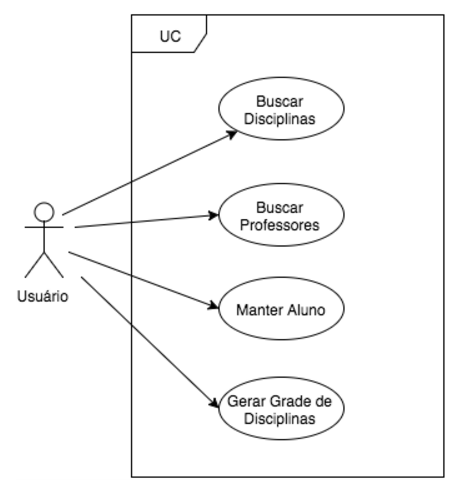
\includegraphics[width=0.6\textwidth]{imagens/modelagemUC}
	\caption{Modelagem de Casos de Uso}
	\label{img:modelagemUC}
\end{figure}

% subsection modelagem_de_casos_de_uso (end)